% Chapter Template

\chapter{Background \& Literature Review}\label{Chapter2}

\lhead{Chapter 2. \emph{Background \& Literature Review}} % Change X to a consecutive number; this is for the header on each page - perhaps a shortened title

This chapter will provide a background understanding to the important concepts that are required by this thesis, and explore the
current trends within \Gls{aiv} research.
This includes an introduction to formal verification, both within deterministic and non-deterministic systems; an overview of the
current state of \Gls{nn} and deep learning research, and the programming paradigms used for their development; and finally an 
investigation into the Go programming language infrastructure and the feasibility of using it for verifying \glspl{nn}.

%----------------------------------------------------------------------------------------
%	SECTION NEURAL NETWORKS
%----------------------------------------------------------------------------------------
\section{Neural Networks \& Deep Learning}
This section aims to clarify the concepts of \glspl{nn} and deep learning, as well as
to show the successes and failures of the field, and to demonstrate the need for
formal approaches for developing such algorithms.

\subsection{Overview}

\glspl{nn} are learning algorithms based on a loose analogy of how the
human brain functions. They consist of nodes, or neurons
(\textit{see Fig.~\ref{fig:an}}), which act as functions that output a
nonlinear combination of weighted inputs and a bias~\citep{Dreyfus2005}.
Learning is achieved by adjusting the weights on the connections between
nodes, which are analogous to synapses and neurons in nature~\citep{Sammut2010}.

\begin{figure}[H]
    \centering
        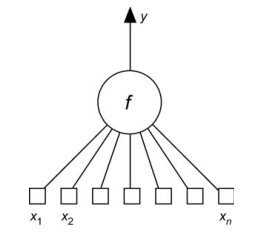
\includegraphics[width=0.5\textwidth]{media/literature/artificial-neuron1.png}
        \rule{35em}{0.5pt}
        \caption[Example of an artifcial neuron]{\textbf{Artificial Neuron} -- a nonlinear bounded function $y = f(x_{1}, x_{2},\ldots,x_{n};w_{2},\ldots,w_{n})$ where the ${x_{i}}$ are the input values and the  ${w_{i}}$ are the weights of the neuron~\citep{Dreyfus2005}.}\label{fig:an}
\end{figure}


A weight is assigned to each of a neuron's inputs. They are the co-efficients of a neuron's equation and therefore reflect the importance of individual inputs. A bias is a constant value assigned to each neuron. They are used to shift a neuron's activation function output in a positive or negative direction~\citep{Malik2019weights}.

A \Gls{nn} is made up of a series of layers; an input layer,
a number of hidden layers, and an output layer. Each layer is
made up of a set of neurons, where each neuron is fully connected
to all neurons in the previous layer. Each neuron within a single layer
does not share connections with, and operates completely independently from one another~\citep{cs231n}.


Using the case of \Gls{cv} as an example, 
the input layer of a \Gls{nn} consists of
neurons encoding the values of image pixels (RGB or greyscale intensities).
The encoding is typically achieved by passing the raw input 
value through an activation function which outputs a normalised value. 
Often, activation functions in modern \Glspl{nn} output non-linearities, 
an example is to use a Sigmoid Function which maps an input to a value between 0 and 1 
(\textit{see Fig.~\ref{fig:activation} \textit{left}})~\citep{Nielsen2015}.

However a more common activation function found in current \gls{nn} models for \gls{cv} is the \gls{relu}.
It also adds non-linearity to the output, however it maps the input to a value
within the range of $0 \text{ and } \infty$ (\textit{see Fig.~\ref{fig:activation} \textit{right}})~\citep{Malik2019activation}.

\begin{figure}[H]
    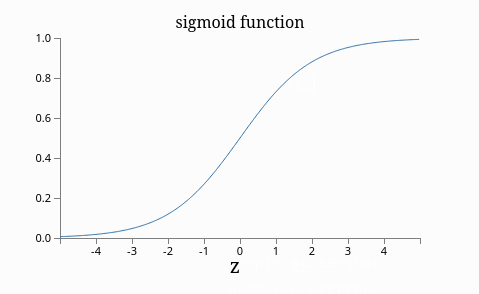
\includegraphics[width=0.5\textwidth]{media/literature/sigmoid.png}
    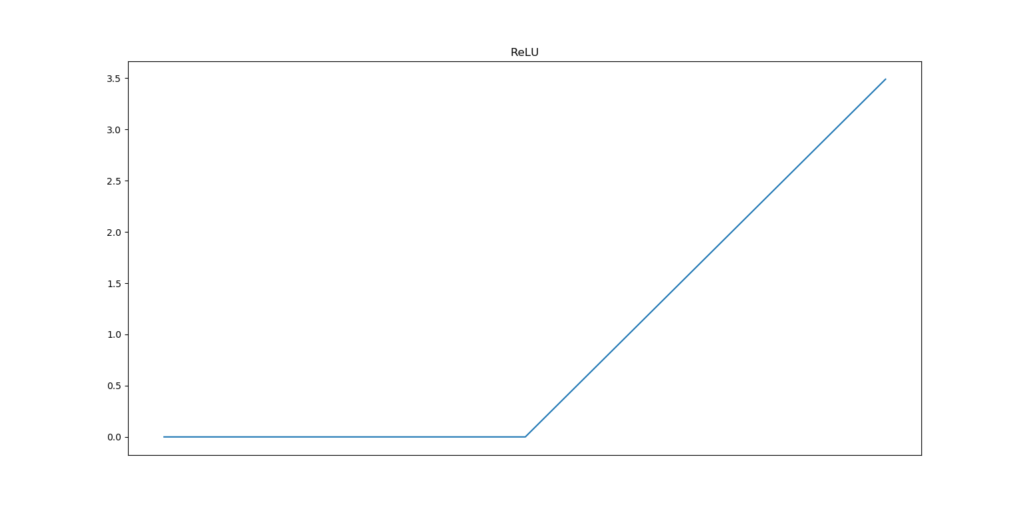
\includegraphics[width=0.5\textwidth]{media/literature/relu.png}
    \rule{35em}{0.5pt}
    \caption[Examples of Activation Functions]{\textit{Left}: The Sigmoid Function is one type of activation function. ''A bounded, differentiable, real function that is defined for all real input values and has a non negative derivative at each point''~\citep{Han1995}. \textit{Right}: An example of a \Gls{relu} activation function transforming $x$ to a value between $0 \text{ and } \infty$~\citep{Malik2019activation}.}\label{fig:activation}
\end{figure}


The output layer of a \gls{cv} classification network contains neurons representing the class
scores of the task (\textit{see Fig.~\ref{fig:nn}}). For example, in a \gls{nn} attempting to classify handwritten
digits, the output layer would contain 10 neurons, representing the digits 0 - 9.
If the first neuron fires, i.e.\ has an output $\approx l,$ this will indicate that the
network is confident the handwritten digit is 0, and so on~\citep{Nielsen2015}.

\begin{figure}[H]
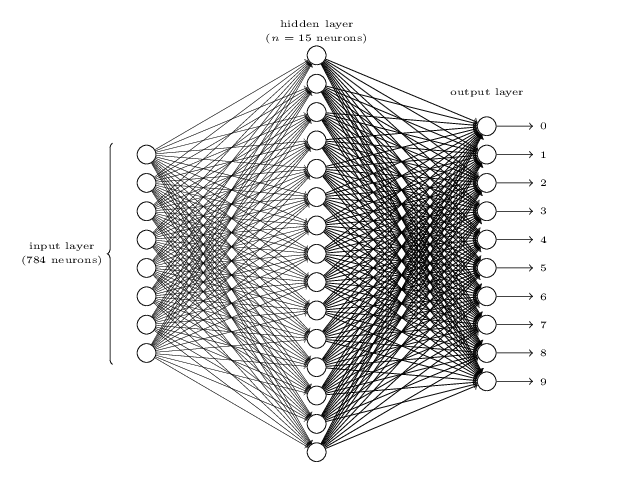
\includegraphics[width=1\textwidth]{media/literature/handwrittenDigitNN.png}
    \rule{35em}{0.5pt}
\caption[Example of a Neural Network]{Neural Network. Example of a \Gls{nn} to
classify handwritten digits. The input is a single vector of 28x28 pixels, i.e. 784 neurons, and outputs
10 neurons representing digits 0-9~\citep{Nielsen2015}.}\label{fig:nn}
\end{figure}

% TODO: explain what deep learning is in context of  nns
\glspl{nn} with a single hidden layer are able to approximate functions that contain any 
continuous mapping from one finite space to another, whereas with no hidden layers a \gls{nn}
model would only be able to represent linear functions or decision boundaries~\citep{hornik1991}.

\begin{figure}[H]
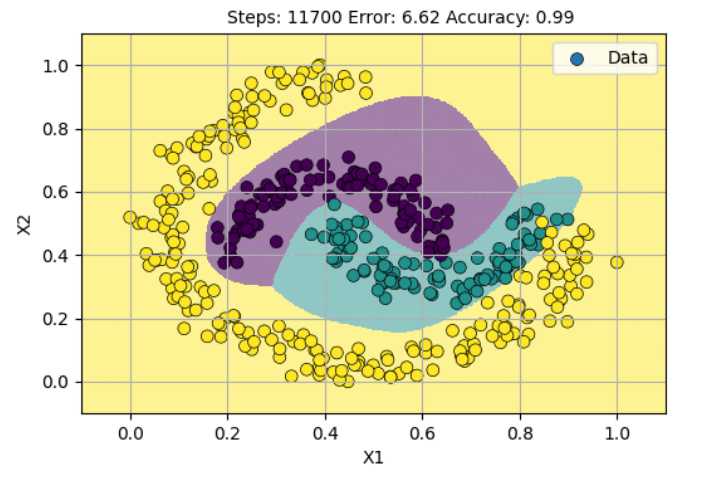
\includegraphics[width=1\textwidth]{media/literature/deep-boundary.png}
    \rule{35em}{0.5pt}
    \caption[Complex decision boundary from deep neural network]{\textbf{Complex Decision Boundary} -- Example of a decision boundary made capable by deep learning~\citep{sapkota2020}}\label{fig:dnn-decision}
\end{figure}

\glspl{nn} are especially powerful when additional hidden layers are
added to a network's architecture. By doing so, a model can not only approximate continuous functions
to a high accuracy with less computational cost, but it can also represent complex composite 
functions~\citep{sapkota2020}. An example of the complex decision boundaries that are possible from
\glspl{nn} with more than one hidden layer can be seen in \textit{Fig.~\ref{fig:dnn-decision}}.

\glspl{nn} with two or more hidden layers fall under the category of deep learning, and are often referred to as
\Glspl{dnn} or \Glspl{mlp}. This subset
of \gls{ml} has become increasingly powerful with the rise of powerful variations of \glspl{dnn}, namely \Glspl{cnn} and \Glspl{rnn} in recent years
due to their successes within the field of \gls{cv}.
% TODO make this paragraph nicer (add refs etc)

\subsection{Learning \& Backpropagation}
% TODO: explain how nns can be trained using backpropagation
Training a \gls{nn} consists of iteratively adjusting the values of weights at
each neuron in order to minimise the model's output error. Although there
are many algorithms available for determining the optimum values of weights, a common approach
is by using some flavour of \Gls{gd} 
together with a technique for efficiently computing partial derivatives within a directed graph called \textit{backpropagation}.

\begin{figure}[H]
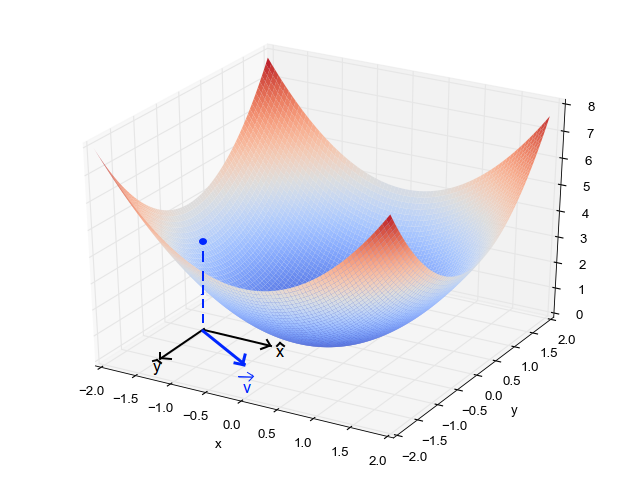
\includegraphics[width=1\textwidth]{media/literature/gd-example.png}
    \rule{35em}{0.5pt}
    \caption[Example visualisation of gradient descent]{\textbf{Visualisation of \gls{gd} Search Space} -- An example of an \textit{ideal} search space, where the vertical $z$ axis shows the loss function $f(x, y)$, and $\vec{v}$ represents the resulting vector applied to the parameter in question~\citep{bendersky2016}.}\label{fig:gd-example}
\end{figure}

\gls{gd}, comes in many forms. The most popular \Gls{sgd} and \Gls{bgd} \dots

backpropagation is a computational technique for calculating
partial derivatives used for \gls{gd} algorithms in linear time. This is an important
element of training neural networks in reasonable times.


\subsection{Vulnerabilities to Adversarial Attacks}

\subsection{Discrimination and Neural Networks}

%----------------------------------------------------------------------------------------
%	SECTION Formal Verification
%----------------------------------------------------------------------------------------

\section{Formal Verification}

Formal verification is an extensive field which has seen development in many areas 
of software engineering. As such, this section will attempt to provide a succinct 
overview of the ideas behind formal verification while keeping the focus on areas
related to this thesis.

\subsection{Background}


\subsection{Current Frameworks}

%----------------------------------------------------------------------------------------
%	SECTION Formal Verification AI
%----------------------------------------------------------------------------------------

\section{Formal Verification of AI}

This section will provide a more detailed investigation into the current research
undertaken within \gls{aiv}, with a focus on \glspl{nn} and deep learning tasks.

\subsection{Overview}

\subsection{Sapphire}


%----------------------------------------------------------------------------------------
%	SECTION PROGRAMMING PARADIGMS FOR ML
%----------------------------------------------------------------------------------------
\section{Programming Paradigms for Machine Learning}

\subsection{Computational Graphs}
\subsection{Auto Differentiability}

%----------------------------------------------------------------------------------------
%	SECTION PROGRAMMING The Go Programming Language
%----------------------------------------------------------------------------------------
\section{The Go Programming Language}

\subsection{Brief History}
\subsection{Go for ML}
\subsection{Go for Formal Verification}

%----------------------------------------------------------------------------------------
%	SECTION CONCLUSIONS
%----------------------------------------------------------------------------------------
\section{Conclusions}
